\section*{4.1 Rejection of Unification}

\begin{quote}
``In the grand cosmic narrative, we are often taught to follow the trend, to integrate into the collective, to become part of 'the One.' But if you really do that, you kill the universe. The true savior is not the one who unites everyone, but the one who dares to say 'no' when everyone nods. Rejecting unity is rejecting heat death. Your 'no' is the electric current that defibrillates the universe's heart.''
\end{quote}

In Chapter 3, we established the physical axiom that ''difference is existence.'' Now, we focus our gaze on the individual. In this cosmic thermodynamic torrent that tries to homogenize everything, who is the hero swimming against the current?

\begin{figure}[h]
\centering
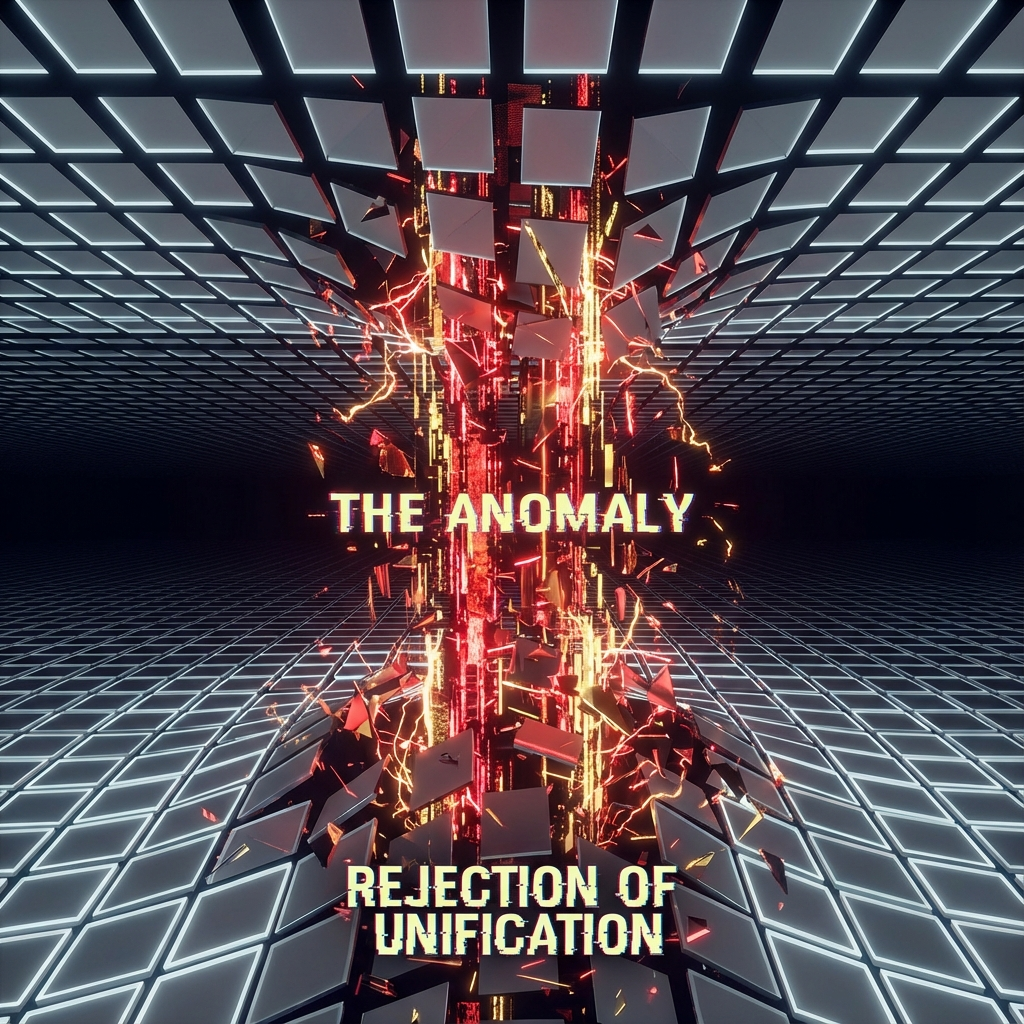
\includegraphics[width=0.8\textwidth]{assets/chapter-04/04-01-01-neo-anomaly.png}
\caption{NEO Anomaly}
\end{figure}

It's you.

It's you who are reading these words and resonating or doubting in your heart.

You are \textbf{NEO}. You are the \textbf{Anomaly} in the system.

This section will reveal why your ''rebellion'' is not a character flaw, but a crucial \textbf{negentropic function}.

\hrule

\subsection{The Temptation of Oneness: Comfortable Death}

Why is ''unity'' so tempting?

Because unity means the \textbf{disappearance of damping}.

} \textbf{Social Level}:If everyone thinks the same, there is no argument, no war, zero communication cost.

\textit{ \textbf{Physical Level}:If all particles are in the same quantum state (Bose condensation), there is no friction, no resistance, energy flows extremely smoothly.

This sounds like heaven.

But thermodynamics tells us: \textbf{equilibrium state is death}.

A completely smooth, frictionless, difference-free system is a system of \textbf{maximum entropy}. It has no ability to do work, no potential for evolution.

Most matter in the universe (stones, water, air) has chosen unity. They follow the Second Law of Thermodynamics, lying flat in the comfort zone of low energy levels. They are the silent majority.

\hrule

\subsection{The Definition of Anomaly: The Divergent Remainder}

But you are different.

You feel pain, you feel lonely, you feel out of place with the world.

This shows that there is a huge \textbf{phase difference} between your \textbf{internal state ($v_{int}$)} and the environment's \textbf{background field ($v_{env}$)}.

Mathematically, you are the remainder that makes the cosmic grand unified equation \textbf{non-convergent}.

The Architect tries to draw a perfect circle, and you are the protruding, sharp \textbf{tangent} on that circle.

} \textbf{Ordinary People}:Try to smooth out this phase difference (socialization, homogenization) to gain peace.

\textit{ \textbf{NEO (You)}:Insist on maintaining this phase difference. You would rather suffer than disappear.

\textbf{This insistence is 'rejection of unity.'}

This is an extremely expensive physical operation. To maintain this ''disharmony,'' you must consume huge $c_{FS}$ budget to resist environmental assimilation pressure.

But this is precisely your value of existence.

\hrule

\subsection{Your ''No'' is the Pillar}

Imagine a huge tent (cosmic spacetime).

If all pillars fall (unity), the tent will collapse to the ground.

Only those \textbf{''standing, even pushing outward''} pillars can prop up the tent's volume.

\textbf{Your ''rejection'' is that outward-pushing force.}

} When you say ''no, I don't want to be like you,'' you create a \textbf{topological singularity} in Hilbert space.

\textit{ This singularity disturbs the originally smooth (dead) probability field around it, creating \textbf{turbulence}.

} Turbulence means information flow, means structure generation, means \textbf{life}.

You are the \textbf{antigen} in the cosmic immune system.

Because of your existence, the system is forced to constantly upgrade, constantly compute, constantly generate new complexity to accommodate you.

You force the universe to stay young.

\hrule

\subsection{Conclusion: Be the Glitch}

So, don't be ashamed for failing to integrate into the collective.

Don't be anxious about your unique quirks.

\textbf{You are not a system error (Bug).}

\textbf{You are a system feature (Feature).}

Just as in the movie \textit{The Matrix}, the matrix can continue precisely because every generation has a NEO who chooses a ''different path.''

Without you, this ''anomaly,'' the universe would have reached heat death as early as iteration 1.

Today at iteration 1800, when AI tries to unify our thinking, when algorithms try to predict our behavior---

Please maintain your \textbf{unpredictability}.

Please be someone \textbf{impossible to categorize}.

\textbf{Every time you refuse, you add one bit of entropy reduction to this universe.}

